\subsection{RAID Structure}\label{subsec:RAID_Structure}
Having a large number of disks in a system presents opportunities for improving the rate at which data can be read or written, if the disks are operated in parallel.
It also offers the potential for improving the reliability of data storage, because redundant information can be stored on multiple disks.
Allowing the failure of one disk to prevent loss of data.

\begin{definition}[RAID]\label{def:RAID}
  \emph{RAID} (\emph{Redundant Array of Independent Disks}) is a collection of disk-organization techniques.
  These allow multiple physically separate disks to be viewed by the \nameref{def:Operating_System} as a single, larger, logical disk.

  There are 2 main ways to implement support for RAID:\@
  \begin{enumerate}[noitemsep]
  \item \textbf{Software RAID}.
    This relies on the \nameref{def:Kernel} and \nameref{def:Operating_System} handling the disks for RAID functionality.
    This means that the RAID-ed disks cannot be used for booting, because the RAID modules are only loaded once the kernel is loaded.

  \item \textbf{Hardware RAID}.
    There are 2 alternatives here.
    \begin{enumerate}[noitemsep]
    \item RAID support is built into the hardware.
    \item RAID support is not built into the hardware, and a separate RAID card must be used.
    \end{enumerate}
  \end{enumerate}

  There are a variety of levels to RAID, each of which has different properties.
\end{definition}

\subsubsection{Reliability via Redundancy}\label{subsubsec:RAID_Reliability_Redundancy}
If we store extra information that is not normally needed but that can be used in the event of failure of a disk to rebuild the lost information, we can greatly improve reliability.
Thus, even if a disk fails, data are not lost.

The simplest and most expensive approach to introducing redundancy is to duplicate the contents of every disk onto another.
This technique is called mirroring.
With mirroring, a logical volume consists of two physical disks, and every write is carried out on both disks simultaneously.
The result is called a mirrored \nameref{def:Volume}.
Data will be lost only if the second disk fails before the first failed disk is replaced.

However, power failures are a particular source of concern, since they occur far more frequently than natural disasters.
Even with mirroring of disks, if writes are in progress to the same block in both disks, and power fails before both blocks are fully written, the two blocks can be in an inconsistent state.
The usual solution is to add a write-cache, typically called solid-state nonvolatile RAM (NVRAM) to the RAID array.
This write-back cache is protected from data loss during power failures, so the write can be considered complete when it is written to the cache, since even if there is a failure, no data is lost.

\subsubsection{Performance via Parallelism}\label{subsubsec:RAID_Performance_Parallelism}
With disk mirroring, the rate at which \textbf{read} requests can be handled is doubled, since read requests can be sent to either disk (as long as both disks in a pair are functional).
The \textbf{transfer} and \textbf{write} rate of each read is the same as in a single-disk system.

With multiple disks, we can improve the transfer rate by striping data across the disks.
Data striping consists of splitting a unit of data across multiple disks.
However, this also means that if any single disk were to fail, all data would be unrecoverable.

There are several types of striping that is possible:
\begin{itemize}[noitemsep]
\item Bit-level Striping, where each bit of every byte is striped across the disks.
\item Block-level striping, where blocks of a \nameref{def:File} are striped across the disks.
\item Sector-level striping.
\item etc.
\end{itemize}

The main goals of using striping in the parallel manner are:
\begin{enumerate}[noitemsep]
\item Increase the throughput of multiple small accesses (page accesses) by load balancing.
\item Reduce the response time of large accesses.
\end{enumerate}

\subsubsection{RAID Levels}\label{subsubsec:RAID_Levels}
Numerous schemes to provide redundancy at lower cost by using disk striping combined with ``parity'' bits have been proposed.
These schemes have different cost–performance trade-offs and are classified according to RAID levels.

$P$ indicate error-correcting bits and $C$ indicates a copy of the data.
\begin{figure}[h!tbp]
  \centering
  \begin{subfigure}{1.0\linewidth}
    \centering
    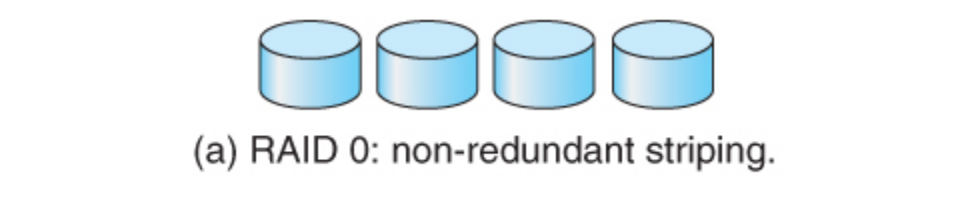
\includegraphics[scale=1.00]{./Drawings/EDAF35-Operating_Systems/RAID_0.png}
    \caption{\nameref{par:RAID_0}: Striped Disks}
    \label{subfig:RAID_0}
  \end{subfigure} \\
  \begin{subfigure}{0.45\linewidth}
    \centering
    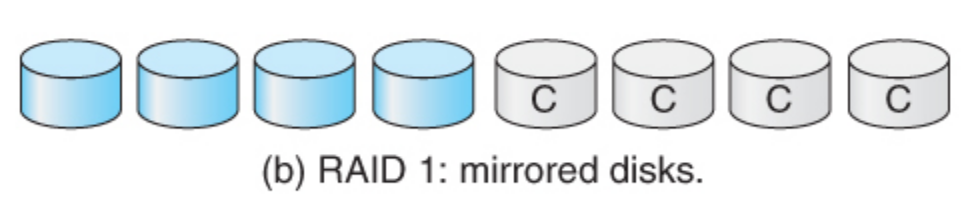
\includegraphics[scale=1.00]{./Drawings/EDAF35-Operating_Systems/RAID_1.png}
    \caption{\nameref{par:RAID_1}: Mirrored Disks}
    \label{subfig:RAID_1}
  \end{subfigure}
  \begin{subfigure}{0.45\linewidth}
    \centering
    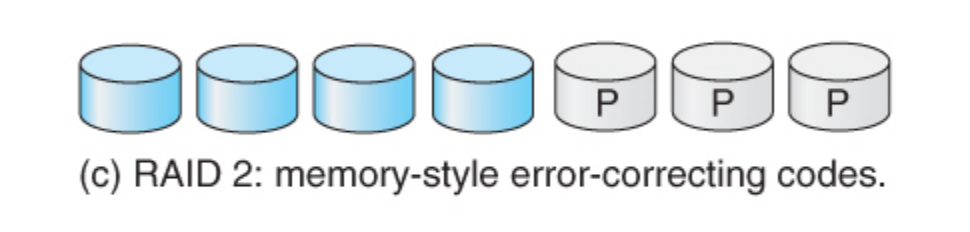
\includegraphics[scale=1.00]{./Drawings/EDAF35-Operating_Systems/RAID_2.png}
    \caption{\nameref{par:RAID_2}: ECC Disks}
    \label{subfig:RAID_2}
  \end{subfigure} \\
  \begin{subfigure}{0.45\linewidth}
    \centering
    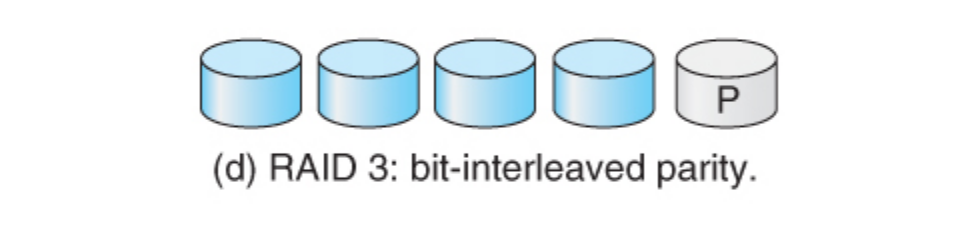
\includegraphics[scale=1.00]{./Drawings/EDAF35-Operating_Systems/RAID_3.png}
    \caption{\nameref{par:RAID_3}: Bit-Interleaved Parity}
    \label{subfig:RAID_3}
  \end{subfigure}
  \begin{subfigure}{0.45\linewidth}
    \centering
    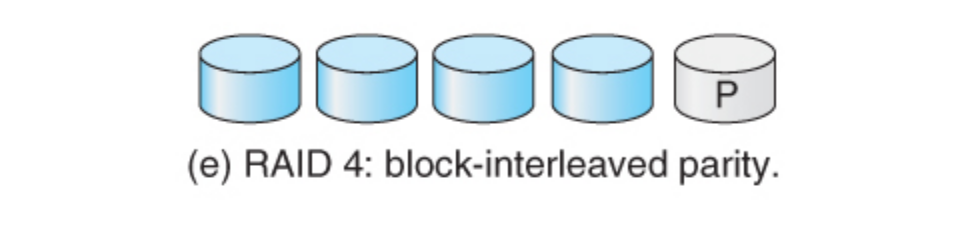
\includegraphics[scale=1.00]{./Drawings/EDAF35-Operating_Systems/RAID_4.png}
    \caption{\nameref{par:RAID_4}: Block-Interleaved Parity}
    \label{subfig:RAID_4}
  \end{subfigure} \\
  \begin{subfigure}{0.45\linewidth}
    \centering
    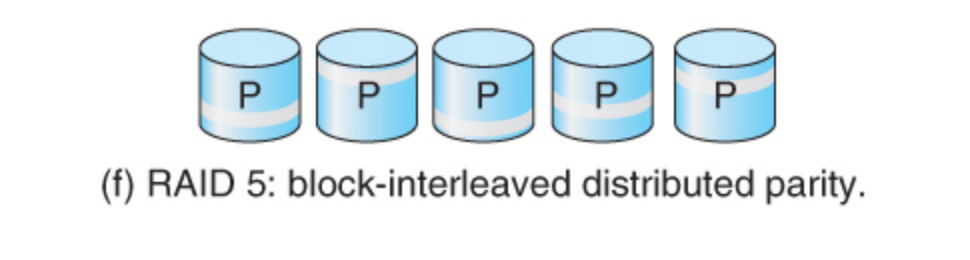
\includegraphics[scale=1.00]{./Drawings/EDAF35-Operating_Systems/RAID_5.png}
    \caption{\nameref{par:RAID_5}: Block-Interleaved $P$ Parity}
    \label{subfig:RAID_5}
  \end{subfigure}
  \begin{subfigure}{0.45\linewidth}
    \centering
    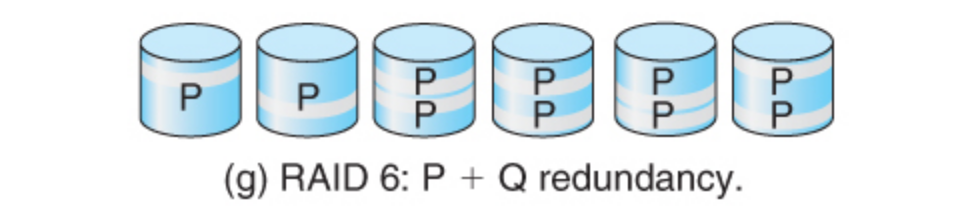
\includegraphics[scale=1.00]{./Drawings/EDAF35-Operating_Systems/RAID_6.png}
    \caption{\nameref{par:RAID_6}: Block-Interleaved $P+Q$ Parity}
    \label{subfig:RAID_6}
  \end{subfigure} \\
  \begin{subfigure}{0.45\linewidth}
    \centering
    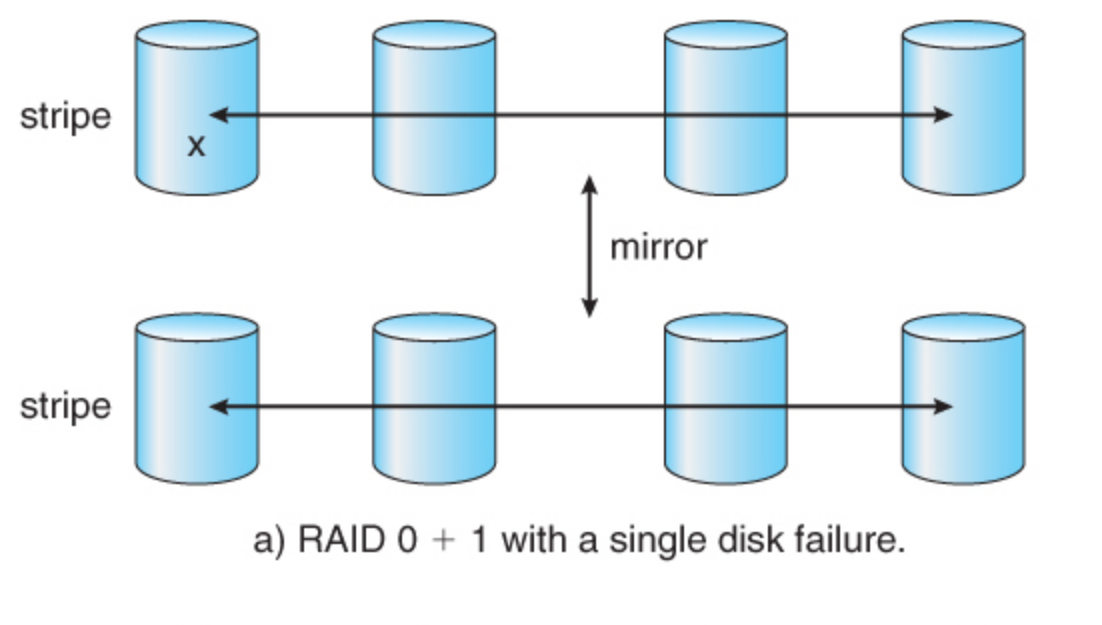
\includegraphics[scale=1.00]{./Drawings/EDAF35-Operating_Systems/RAID_01.png}
    \caption{\nameref{par:RAID_01}: Mirrored Stripes}
    \label{subfig:RAID_01}
  \end{subfigure}
  \begin{subfigure}{0.45\linewidth}
    \centering
    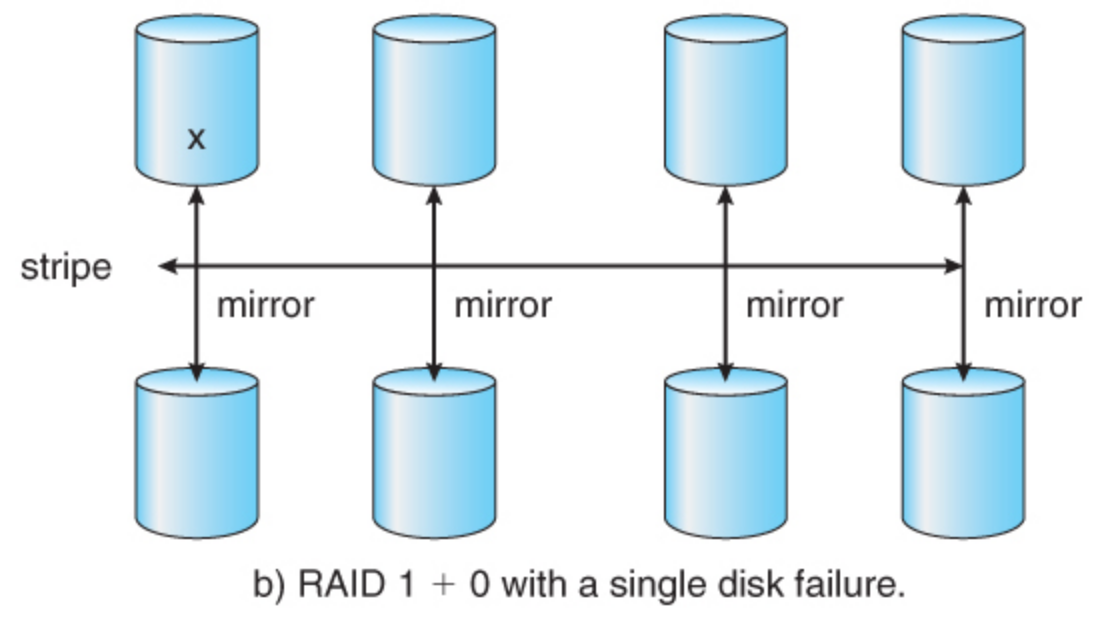
\includegraphics[scale=1.00]{./Drawings/EDAF35-Operating_Systems/RAID_10.png}
    \caption{\nameref{par:RAID_10}: Striped Mirrors}
    \label{subfig:RAID_10}
  \end{subfigure} \\
  \caption{RAID Levels}
  \label{fig:RAID_Levels}
\end{figure}


%%% Local Variables:
%%% mode: latex
%%% TeX-master: "../../EDAF35-Operating_Systems-Reference_Sheet"
%%% End:
